\chapter{Literature Review}\label{ch:literature-review}
\section{Indoor Localisation Systems}\label{sec:indoor-localisation-sensors}
\subsection*{Passive Systems}
In summary, passive systems do not require the object being tracked to have some of electronics on them to do positioning.
Some examples of passive systems are ~\citep{deak2012survey}:
\begin{itemize}
    \item Computer Vision and Imaging systems.
    \item Tactile and contact sensors.
    \item Attenuation of signals.
    \item Differential air pressure.
\end{itemize}
A common example of computer vision based localisation is to use a setup consisting of multiple cameras in a space trying to detecting a single object.
Using the intrinsic and extrinsic properties of each camera it is possible to determine the transform to the object in a given frame with relatively high accuracy.
A prime example of this is the commercial VICON motion capture systems.
~\cite{aerialrobotsiitk} shows a drone application in which the UAV is positioned via using a VICON motion capture system.
Figure~\ref{fig:vs} shows the simplified setup, it should be noted that the UAV must be equipped with specialised marker that is used to identify it.
Furthermore, the positions are fed to a companion computer connected to the autopilot system.
The VICON setup provides highly accurate positions and is often used to gather ground truth positional data to compare to other positioning systems.
The additional requirements of the VICON systems, however, do not make it feasible for indoor applications.

\begin{figure}[h!]
    \centering
    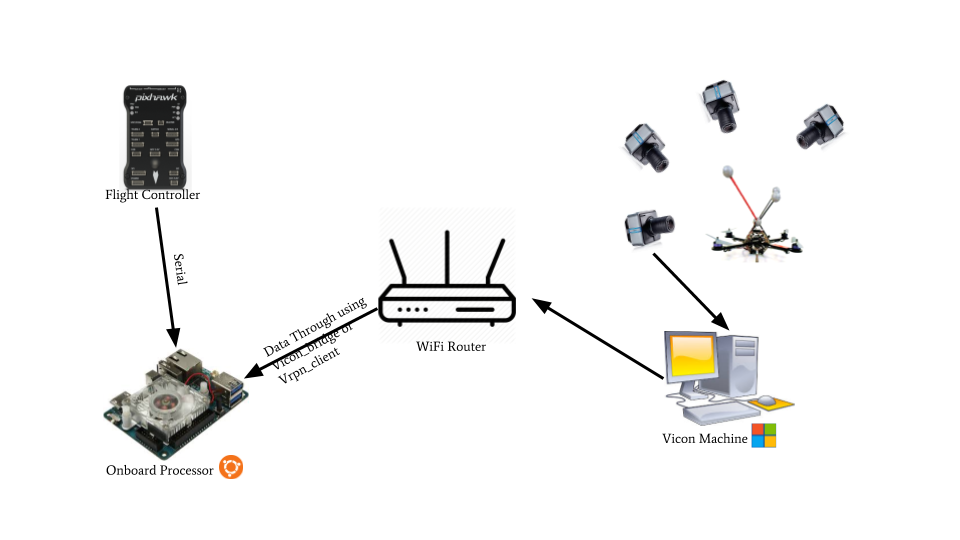
\includegraphics[scale=.45]{vicon_setup}
    \caption{VISON setup for position of a UAV. (\url{https://aerial-robotics-iitk.gitbook.io/wiki/estimation/setup-with-vicon})}
    \label{fig:vs}
\end{figure}

\subsection*{Active Systems}
In contrast to passive systems, active systems have the object being positioned equipped with electronics.
Many indoor localisation techniques use this and some examples are ~\cite{deak2012survey}
\begin{itemize}
    \item Radio-frequency identification
    \item UWB
    \item Wireless Local Area Network
    \item Bluetooth Low energy (BLE)
\end{itemize}
Many of these setups use an anchor and tag configuration.
The tag receives signals from multiple anchors and triangulates the tag.

An approach using and comparing UWB and BLE is developed by ~\cite{findobjs} to do localisation in a museum.
Both methods are combined with a dead reckoning system to improve accuracy.
Six paintings are equipped with both a BLE and UWB tag

\begin{figure}[h!]
    \centering
    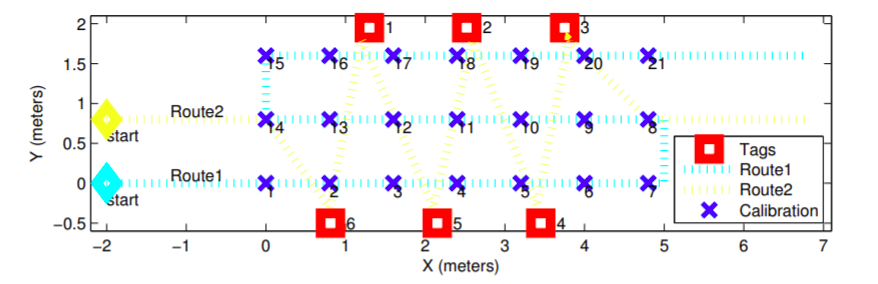
\includegraphics[scale=.45]{uwb_vs_ble}
    \caption{Setup used to compare UWB and BLE performance in a museum.}
    \label{fig:uwbvsble}
\end{figure}

\section{Pozyx - Behind the Scenes}\label{sec:pozyx---behind-the-scenes}
